\documentclass[12pt]{article}
\usepackage[utf8]{inputenc}
\usepackage{amsmath}
\usepackage{graphicx}
\usepackage{geometry}
\usepackage{listings}
\usepackage{caption}
\usepackage{color}

\definecolor{dkgreen}{rgb}{0,0.6,0}
\definecolor{gray}{rgb}{0.5,0.5,0.5}
\definecolor{mauve}{rgb}{0.58,0,0.82}

\lstset{frame=tb,
  language=Matlab,
  aboveskip=3mm,
  belowskip=3mm,
  showstringspaces=false,
  columns=flexible,
  basicstyle={\scriptsize\ttfamily},
  numbers=none,
  numberstyle=\tiny\color{gray},
  keywordstyle=\color{blue},
  commentstyle=\color{dkgreen},
  stringstyle=\color{mauve},
  breaklines=true,
  breakatwhitespace=true,
  tabsize=3
}

\title{EMG$\sigma$-Torque Modeling Using Linear FIR System}
\author{Christian Piper - \texttt{cpiper@wpi.edu}\\ ECE503 - Digital Signal Processing \\ Lab 1}
\date{April 2, 2025}

\begin{document}

\maketitle

\section*{Methods}
This report outlines the methodology for modeling the relationship between surface electromyogram (EMG) standard deviation (EMG$\sigma$) and elbow joint torque using a linear, dynamic finite impulse response (FIR) system. The goal was to develop reproducible MATLAB functions to train and test the model, assessing performance across model orders $Q$ and pseudo-inverse tolerances. Three datasets were utilized: LB1229 (training), LB1249 (test), and LB1269 (spare test). Each dataset begins as raw data recordings from experimental trials, containing three signals: raw extension EMG (biceps), raw flexion EMG (triceps), and torque, originally sampled at 4096 Hz. These raw EMG signals, recorded on the skin, capture muscle electrical activity, while the torque signal measures elbow joint force. To prepare the data, the raw EMG signals are processed to estimate their standard deviation (EMG$\sigma$) by computing the root mean square (RMS) over short time windows, extracting signal intensity correlated with muscle tension. The resulting EMG$\sigma$ estimates and torque are then downsampled to 40.96 Hz, as most torque power resides below 2–3 Hz, yielding the final signals for modeling. The datasets were provided in \texttt{lab1data.mat}, containing structs LB1229, LB1249, LB1269 with fields of the downsampled EMG$\sigma$s: EMGrmsE ($\hat{s}_E[m]$), EMGrmsF ($\hat{s}_F[m]$) and downsampled torque data: T ($T_{Ext}[m]$). The structs also included the original raw data: EMG\_E4096 (raw extensor EMG), EMG\_F4096 (raw flexor EMG), T4096 (raw torque readings), as well as the 4096 Hz EMG$\sigma$s: EMGrmsE4096 (extensor EMG$\sigma$) and EMGrmsF4096 (flexor EMG$\sigma$).

\newpage
\subsection*{Training}
The MATLAB function \texttt{trainFIR} estimates coefficients given preprocessed $\hat{s}_E[m]$, $\hat{s}_F[m]$, $T_{Ext}[m]$, tolerance $Tol$, and $Q$. The first and last 41 samples (1 second at 40.96 Hz) of $\hat{s}_E[m]$, $\hat{s}_F[m]$, and $T_{Ext}[m]$ are trimmed to eliminate filter startup and tail effects from EMG$\sigma$ estimation and downsampling, ensuring stable, artifact-free segments. The FIR model is formulated as a linear regression problem, where the torque output $y[m] = T_{Ext}[m]$ is expressed as $y = A b$, with $y$ being the torque value, $A$ the design matrix, and $b = [e_0, e_1, \ldots, e_Q, f_0, f_1, \ldots, f_Q]^T$ the coefficient vector. For each sample $m$ from $Q+1$ to $N$, the torque is modeled as:
\begin{equation}
y[m] = \sum_{i=0}^{Q} e_i \cdot \hat{s}_E[m-i] + \sum_{i=0}^{Q} f_i \cdot \hat{s}_F[m-i],
\end{equation}
which corresponds to a row in $A$ containing the current and previous $Q$ samples of $\hat{s}_E[m]$ and $\hat{s}_F[m]$. Thus, $A$ is constructed with dimensions $(N-Q) \times 2(Q+1)$:
\begin{equation}
\resizebox{0.9\textwidth}{!}{$ A = \begin{bmatrix} \hat{s}_E[Q+1] & \hat{s}_E[Q] & \cdots & \hat{s}_E[1] & \hat{s}_F[Q+1] & \hat{s}_F[Q] & \cdots & \hat{s}_F[1] \\ \hat{s}_E[Q+2] & \hat{s}_E[Q+1] & \cdots & \hat{s}_E[2] & \hat{s}_F[Q+2] & \hat{s}_F[Q+1] & \cdots & \hat{s}_F[2] \\ \vdots & \vdots & \ddots & \vdots & \vdots & \vdots & \ddots & \vdots \\ \hat{s}_E[N] & \hat{s}_E[N-1] & \cdots & \hat{s}_E[N-Q] & \hat{s}_F[N] & \hat{s}_F[N-1] & \cdots & \hat{s}_F[N-Q] \end{bmatrix} $}
\end{equation}
and $y = [T_{Ext}[Q+1], T_{Ext}[Q+2], \ldots, T_{Ext}[N]]^T$. Since $y = A b$ may not have an exact solution due to noise and model imperfections, the coefficients $b$ are solved by minimizing the squared error $||A b - y||^2$. This least squares problem is addressed using the Moore-Penrose pseudo-inverse $A^\dagger$, yielding:
\begin{equation}
b = A^\dagger \cdot y,
\end{equation}
where $A^\dagger = (A^T A)^{-1} A^T$ (if $A^T A$ is invertible).

\begin{center}
     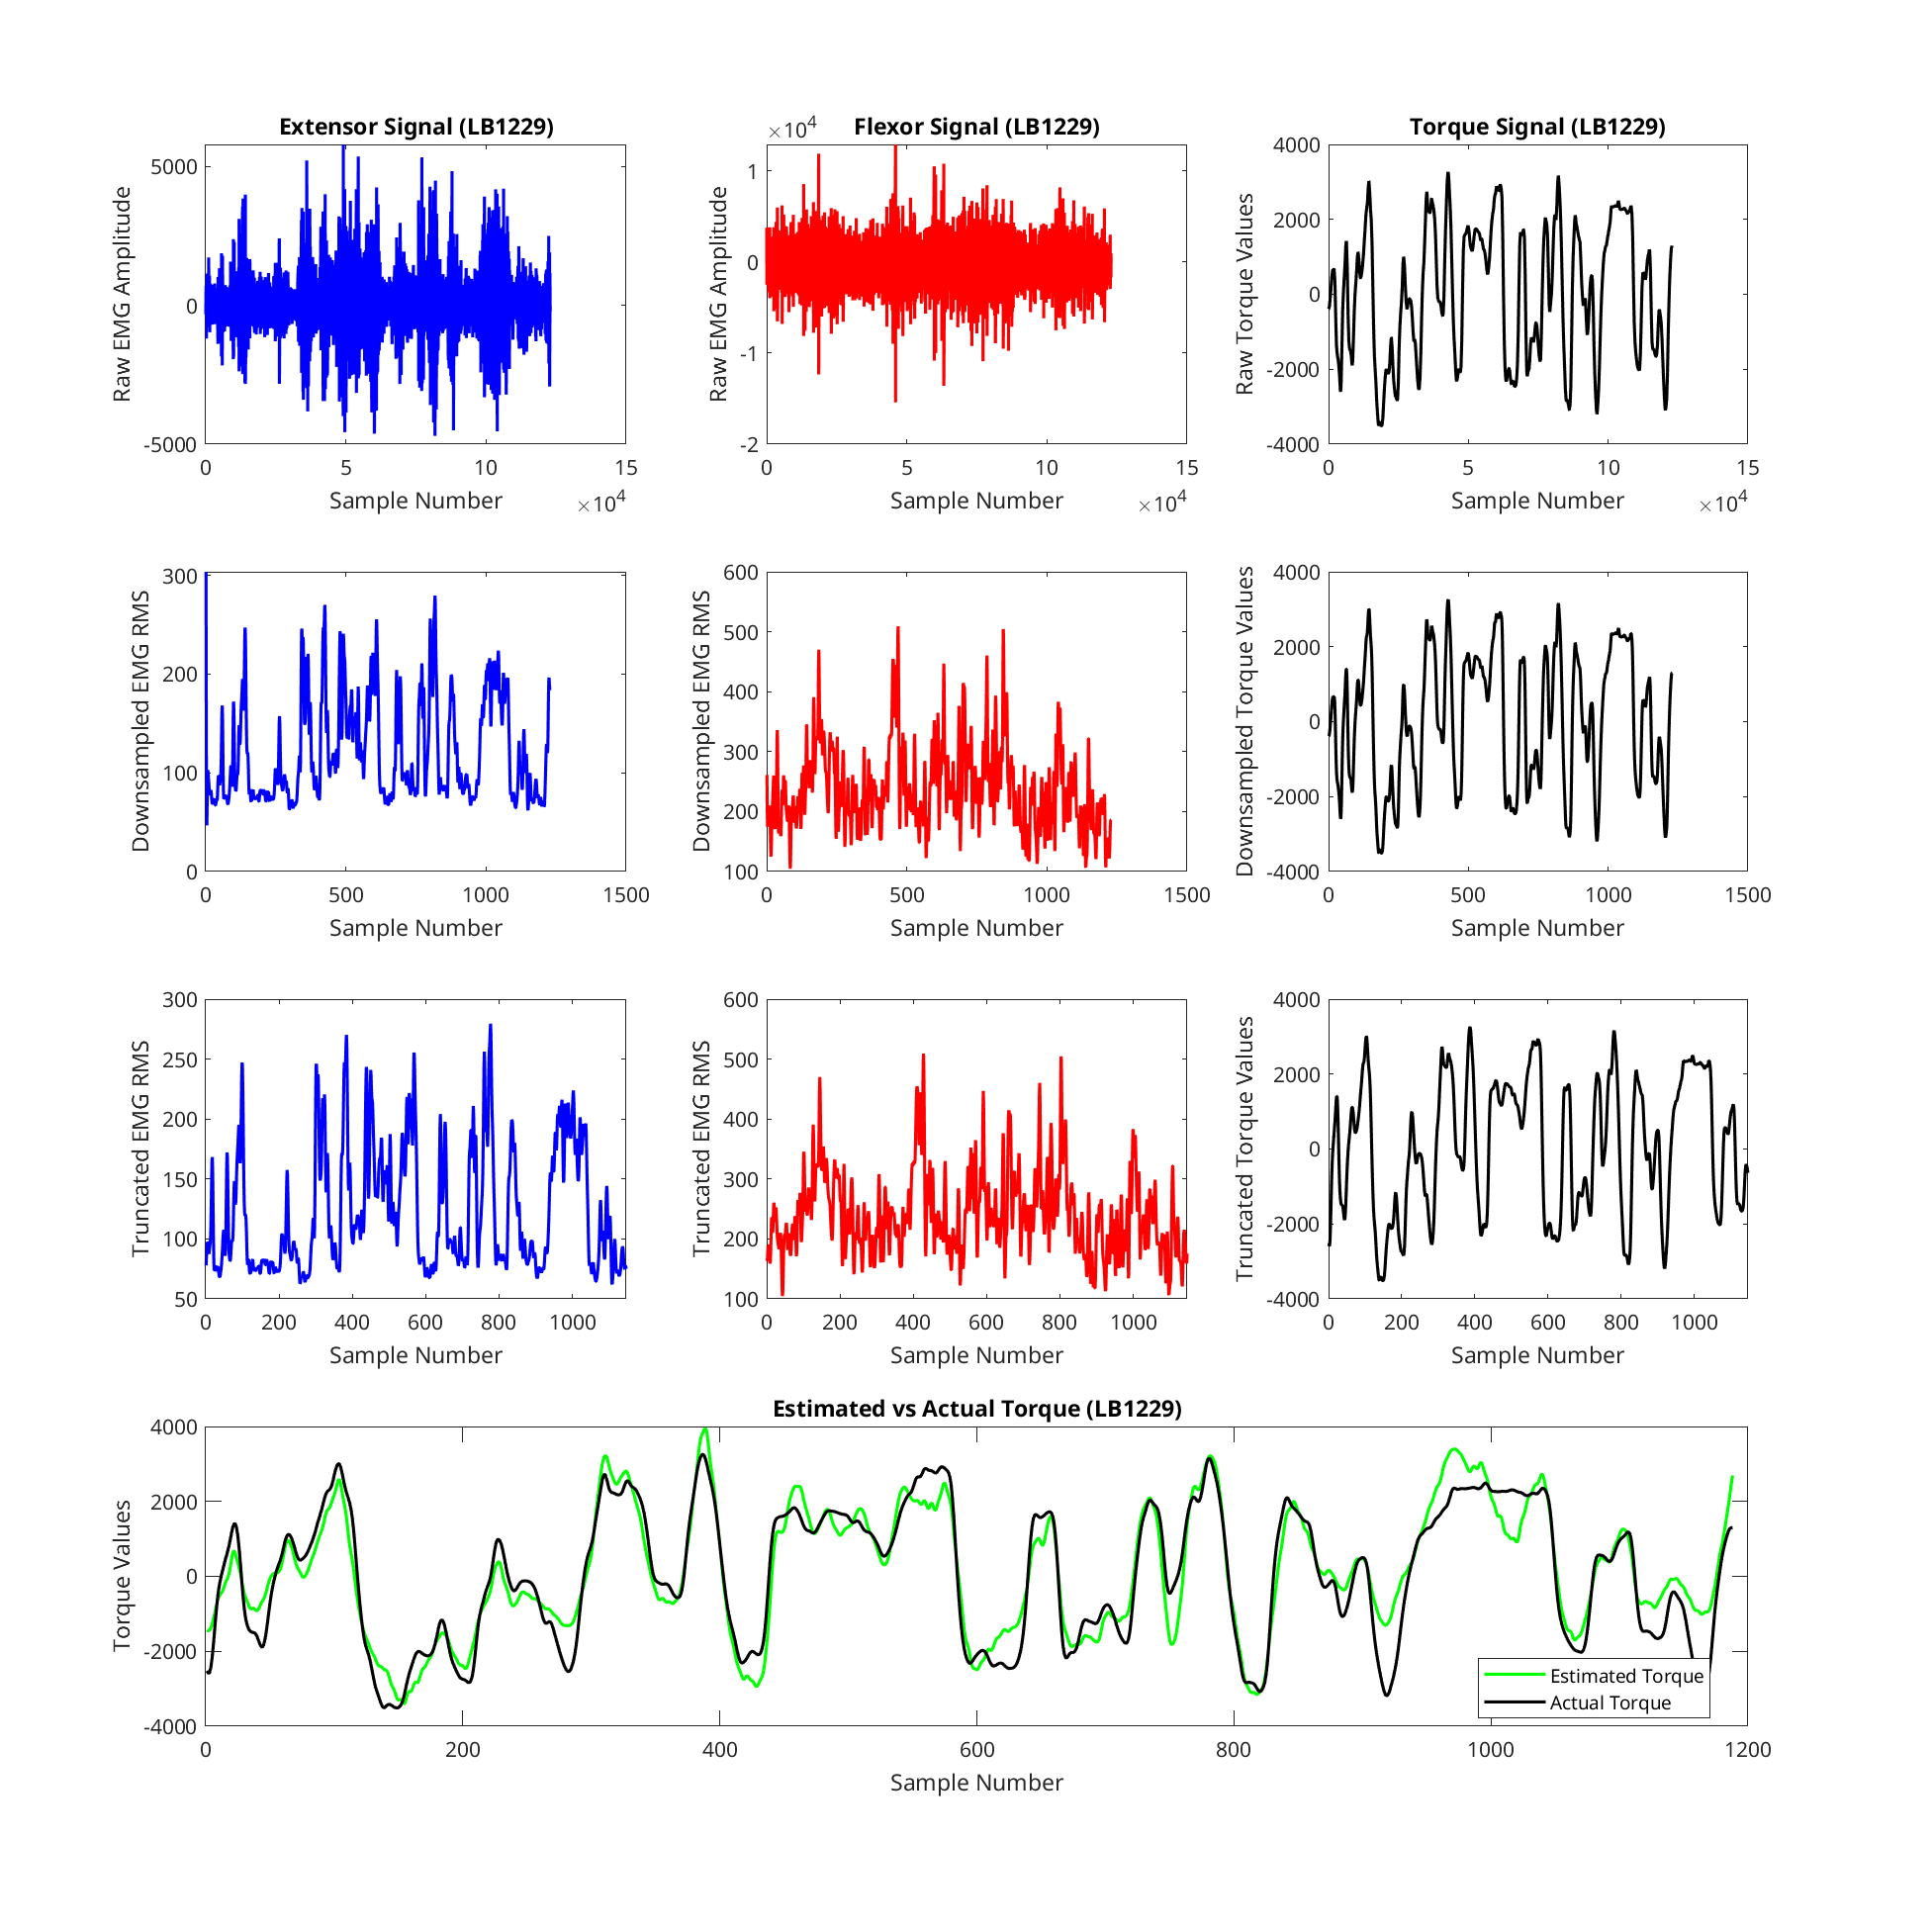
\includegraphics[width=1\textwidth]{plots/lab1_training_overview.png} \\
     \textit{An overview of the training process using the LB1229 dataset, from raw data to torque estimates. EMG values are in ADC units and torque in raw sensor values.}
\end{center}

\newpage
\subsection*{Testing}
The \texttt{testFIR} function evaluates the model using the EMG$\sigma$ estimates ($\hat{s}_E[m]$, $\hat{s}_F[m]$), torque ($T_{Ext}[m]$), and training coefficients. The first 205 samples (5 seconds at 40.96 Hz, adjusted by the model order $Q$) of $\hat{s}_E[m]$, $\hat{s}_F[m]$, and $T_{Ext}[m]$ are removed to avoid startup transients. This ensures consistent evaluation across varying $Q$ values, focusing on stable data segments. The estimated torque is represented by:
\begin{equation}
\hat{T}_{Ext}[m] = \sum_{i=0}^{Q} e_i \cdot \hat{s}_E[m-i] + \sum_{i=0}^{Q} f_i \cdot \hat{s}_F[m-i],
\end{equation}
for $m = Q+1$ to $N$. RMS error is:
\begin{equation}
\text{RMS Error} = \sqrt{\frac{1}{N-Q} \sum_{m=Q+1}^{N} (T_{Ext}[m] - \hat{T}_{Ext}[m])^2}.
\end{equation}

\subsection*{Performance Analysis}
Performance of the EMG$\sigma$-Torque FIR model was evaluated using two distinct MATLAB scripts, detailed in the Appendix, to assess the effects of model order $Q$ and pseudo-inverse tolerance $Tol$ on prediction accuracy. 

The first script, \texttt{generate\_train\_test.m}, analyzes model performance across $Q = 1$ to 200 with a fixed $Tol = 0.005$. It trains the model on LB1229 using \texttt{trainFIR}, then computes RMS errors on LB1229 (training), LB1249 (test), and LB1269 (spare test) via \texttt{testFIR}. The script generates two plots: one comparing training and LB1249 test errors, and another comparing training and LB1269 test errors, both saved as \texttt{lab1\_train\_test\_49.png} and \texttt{lab1\_train\_test\_69.png}, respectively, to visualize overfitting trends as $Q$ increases. 

The second script, \texttt{generate\_tol\_test.m}, explores a grid of $Q = 1$ to 40 and $Tol = 0.0025$ to 0.3 (in 0.0025 increments), training on LB1229 and testing on LB1249 and LB1269. It produces 3D scatter plots of RMS error versus $Q$ and $Tol$ for each test set, saved as \texttt{lab1\_tol\_test\_49.png} and \texttt{lab1\_tol\_test\_69.png}, to examine how tolerance impacts model regularization and fit. Together, these scripts provide a comprehensive analysis of model behavior across key parameters, with results visualized in the subsequent Results section.

\newpage
\section*{Results}
Results are presented in two parts: error versus model order at fixed tolerance, and error versus model order and tolerance.

\subsection*{Error vs. Model Order ($Tol = 0.005$)}
Training on LB1229 and testing on all datasets over $Q = 1$ to 200 yielded: 
\begin{center}
     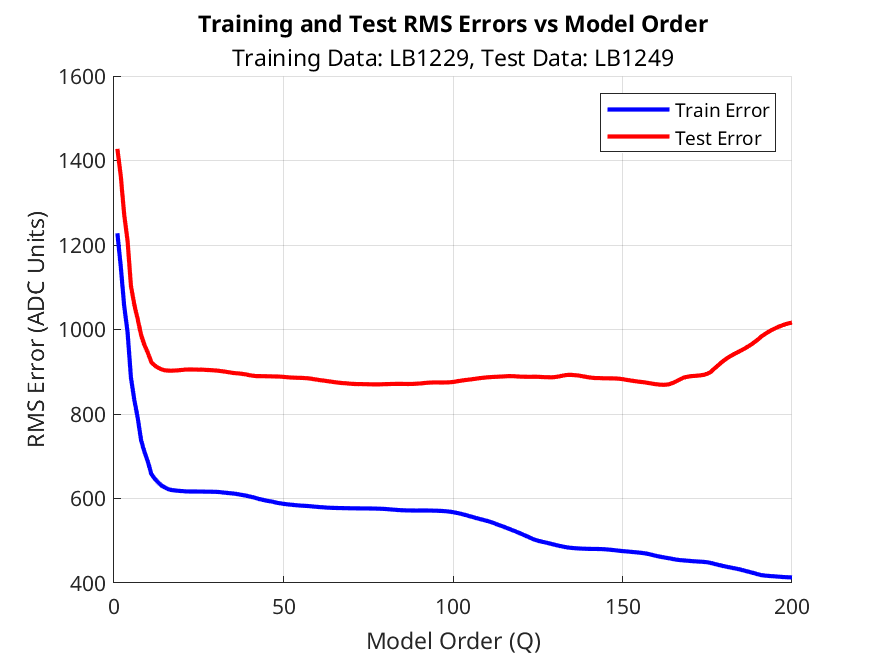
\includegraphics[width=0.8\textwidth]{plots/lab1_train_test_49.png} \\
     \textit{RMS error vs. model order $Q$ for training (LB1229) and test (LB1249) datasets.}
\end{center}
Training error decreased, while test error on LB1249 flatlined around $Q = 20$ (RMS error approximately 900 ADC units), then increased, indicating overfitting. 
\\\\

\begin{center}
     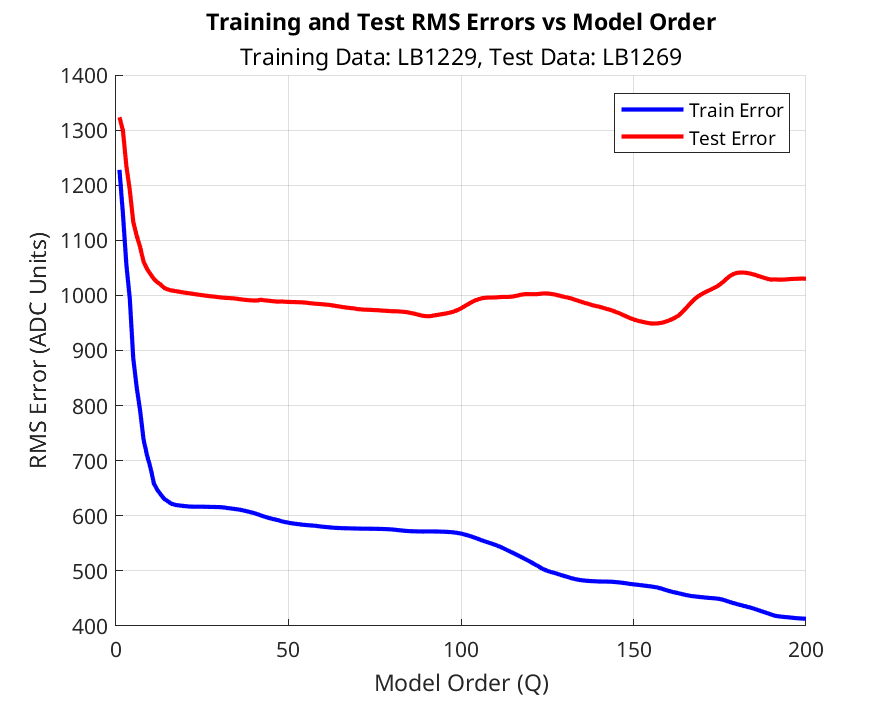
\includegraphics[width=0.8\textwidth]{plots/lab1_train_test_69.png} \\
     \textit{RMS error vs. model order $Q$ for the training (LB1229) and test (LB1269) datasets.}
\end{center}

LB1269 showed a similar trend, with slower error reduction starting around $Q = 20$ (RMS error approximately 1000 ADC units). While error continued to decrease after $Q = 20$, the reduction was likely due to overfitting. The LB1229 training and LB1269 test datasets likely have inherent similarities in their random noise.

\newpage
\subsection*{Error vs. Model Order and Tolerance}
For $Q = 1$ to 40 and $Tol = 0.0025$ to 0.3 in increments of 0.0025, 3D scatter plots were generated. 

\begin{center}
     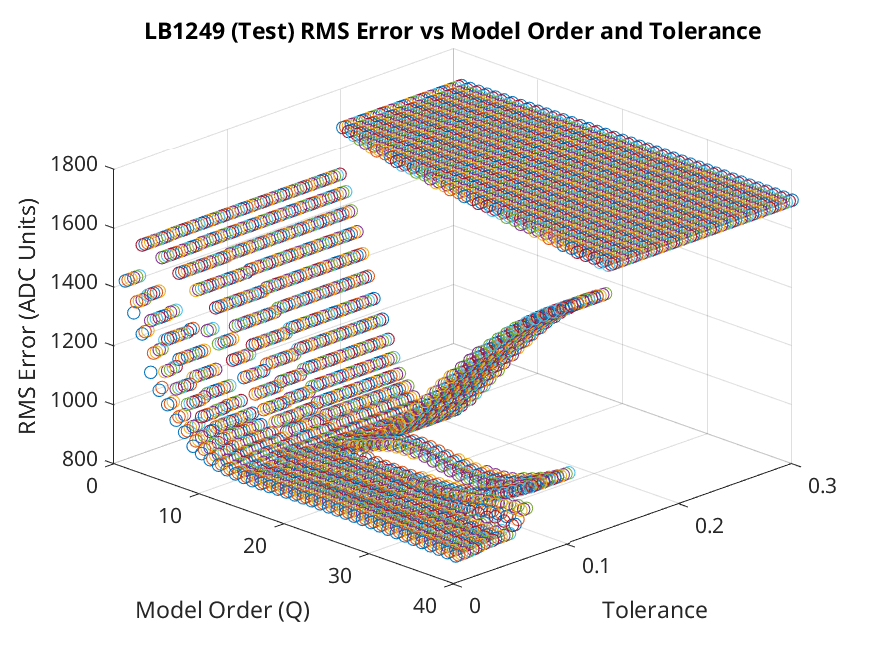
\includegraphics[width=0.8\textwidth]{plots/lab1_tol_test_49.png} \\
     \textit{RMS error vs. model order $Q$ and pseudo-inverse tolerance $Tol$ for training (LB1229) and test (LB1249) datasets.}
\end{center}
Lower tolerances showed a better fit up until around $Tol \approx 0.005$, with the error increasing at higher $Tol$. Varying the model order had similar effects to the previous testing. Error decreases drastically, then flatlines as the model begins to overfit.

\begin{center}
     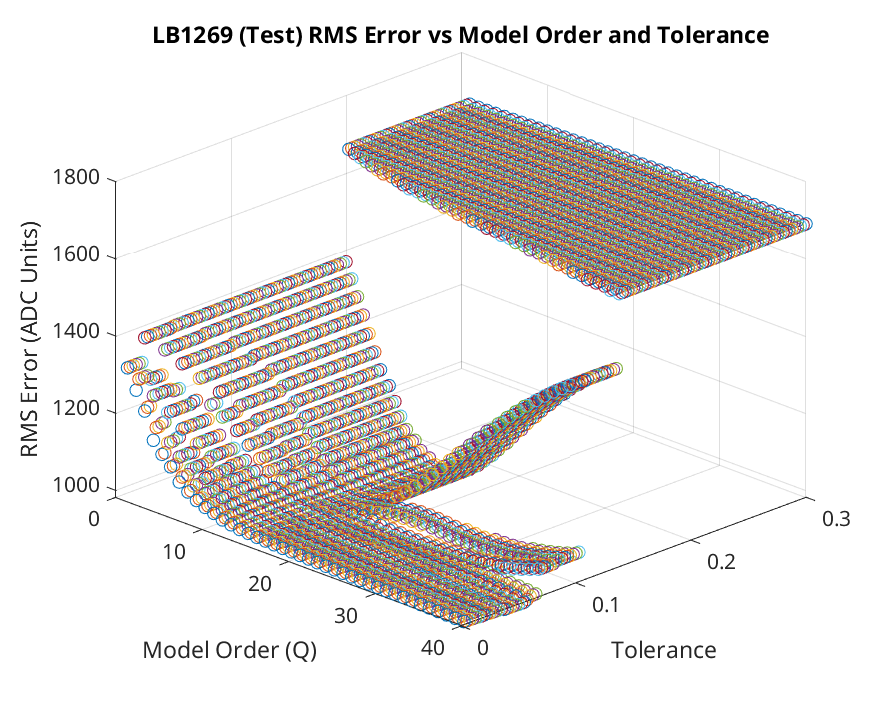
\includegraphics[width=0.8\textwidth]{plots/lab1_tol_test_69.png} \\
     \textit{RMS error vs. model order $Q$ and pseudo-inverse tolerance $Tol$ for training (LB1229) and test (LB1269) datasets.}
\end{center}
LB1269 exhibited comparable behavior, with optimal performance at moderate $Q$ and low $Tol$.

\newpage
\section*{Discussion}
The model effectively captured EMG$\sigma$-torque dynamics, with optimal $Q$ around 20 depending on the test set. Overfitting at high $Q$ reflects noise fitting, while tolerance variation showed that $Tol \approx 0.005$ balances fit and generalization. The slightly lower error of LB1269 suggests better alignment with the dynamics of LB1229.

Several limitations hinder these results. The use of limited number of datasets restricts the model’s applicability to broader populations, as inter-subject variability in muscle activation or sensor placement could alter EMG$\sigma$-torque relationships. Fixed preprocessing—RMS windowing and downsampling to 40.96 Hz—may also miss higher-frequency dynamics or introduce artifacts, particularly if the RMS window is suboptimal for capturing muscle activity. Additionally, the linear FIR assumption simplifies the inherently non-linear relation of EMG readings to muscle force, potentially capping predictive accuracy.

Future work could address these by incorporating non-linear terms (e.g., polynomial or neural network models) to better model the EMG-torque relationship, or by training and testing across a larger number of datasets to enhance robustness. Adaptive RMS window sizes or filtering might also improve signal representation. This analysis revealed that while the FIR model is computationally efficient and produces decent predictions, its performance hinges critically on parameter selection ($Q$, $Tol$), with overfitting posing a key challenge at higher complexity.

\section*{Conclusion}
The FIR model successfully predicted the torque, with optimal performance at $Q \approx 20$ and $Tol \approx 0.005$, validated by independent test sets LB1249 and LB1269.

\newpage
\section*{Appendix}
MATLAB functions are listed below.

\begin{lstlisting}[caption={trainFIR.m}]
function [e, f] = trainFIR(e_rms, f_rms, torque, tol, Q)
    % trainFIR - Trains FIR filter coefficients for a given system.
    %
    % Syntax:
    %   [e, f] = trainFIR(e_rms, f_rms, torque, tol, Q)
    %
    % Inputs:
    %   e_rms   - Vector of RMS values for the extensor signal.
    %   f_rms   - Vector of RMS values for the flexor signal.
    %   torque  - Vector of measured actual torque values (output signal).
    %   tol     - Tolerance for the pseudo-inverse computation.
    %   Q       - Order of the FIR filter (number of previous samples to consider).
    %
    % Outputs:
    %   e       - FIR filter coefficients for the extensor input signal (e_rms).
    %   f       - FIR filter coefficients for the flexor input signal (f_rms).
    %
    % Description:
    %   This function computes the FIR filter coefficients for a system with two
    %   input signals (e_rms and f_rms) and one output signal (torque). It removes
    %   transient samples from the beginning and end of the input and output data,
    %   constructs a regression matrix (A) using the current and previous Q samples
    %   of the input signals, and solves for the filter coefficients using a
    %   pseudo-inverse approach with a specified tolerance.

    % Transient samples (to be removed from beginning and end of data)
    transient_samples = 41; % Number of samples to ignore at the beginning and end

    % Drop the transients
    e_rms = remove_transients(e_rms, transient_samples);
    f_rms = remove_transients(f_rms, transient_samples);
    torque = remove_transients(torque, transient_samples);

    N = length(e_rms);

    % Build the A matrix
    A = zeros(N - Q, 2 * (Q + 1));

    for i = 1:N - Q
        % Create a row of the A matrix using the current and previous Q samples
        A(i, :) = [flip(e_rms(i:i + Q)), flip(f_rms(i:i + Q))];
    end

    % Compute the b vector
    b = pinv(A, tol * norm(A)) * torque(Q + 1:N)';

    % Extract the coefficients for e and f
    e = b(1:Q + 1)';
    f = b(Q + 2:2 * Q + 2)';

end
\end{lstlisting}

\begin{lstlisting}[caption={testFIR.m}]
 function RMS_error = testFIR(e_rms, f_rms, torque, e_coeff, f_coeff)
    % testFIR - Computes the Root Mean Square (RMS) error between the actual torque
    %           and the estimated torque using FIR filter coefficients.
    %
    % Syntax:
    %   RMS_error = testFIR(e_rms, f_rms, torque, e_coeff, f_coeff)
    %
    % Inputs:
    %   e_rms    - Array of RMS values for the extensor signal.
    %   f_rms    - Array of RMS values for the flexor signal.
    %   torque   - Array of measured actual torque values.
    %   e_coeff  - Coefficients for the FIR filter applied to the extensor signal (e_rms).
    %   f_coeff  - Coefficients for the FIR filter applied to the flexor signal (f_rms).
    %
    % Outputs:
    %   RMS_error - The Root Mean Square error between the actual torque and the
    %               estimated torque.
    %
    % Description:
    %   This function calculates the RMS error between the actual torque and the
    %   estimated torque. The estimation is performed using FIR filter coefficients
    %   applied to the input signals (e_rms and f_rms). The function removes transient
    %   samples from the beginning and end of the input data to ensure accurate
    %   calculations. The estimated torque is computed by convolving the input signals
    %   with their respective FIR filter coefficients.
    %
    % Example:
    %   e_rms = [1.2, 1.3, 1.4, ...]; % Example RMS values for signal e
    %   f_rms = [0.8, 0.9, 1.0, ...]; % Example RMS values for signal f
    %   torque = [10, 12, 14, ...];   % Example actual torque values
    %   e_coeff = [0.1, 0.2, 0.3];    % Example FIR coefficients for e_rms
    %   f_coeff = [0.4, 0.5, 0.6];    % Example FIR coefficients for f_rms
    %   RMS_error = testFIR(e_rms, f_rms, torque, e_coeff, f_coeff);

    % Transient samples (to be removed from beginning and end of data)
    transient_samples = 41 * 5; % Number of samples to ignore at the beginning and end
    Q = length(e_coeff) - 1;

    % Drop the startup transients
    e_rms = remove_startup_transients(e_rms, transient_samples - Q);
    f_rms = remove_startup_transients(f_rms, transient_samples - Q);
    torque = remove_startup_transients(torque, transient_samples - Q);

    N = length(e_rms);

    % Estimate the torque using the coefficients
    estimated_torque = zeros(1, N - Q);

    for i = 1:N - Q
        % Calculate the estimated torque for each sample using the coefficients
        estimated_torque(1, i) = sum(e_coeff .* flip(e_rms(i:i + Q))) + sum(f_coeff .* flip(f_rms(i:i + Q)));
    end

    RMS_error = sqrt(mean((torque(Q + 1:N) - estimated_torque) .^ 2));
end
\end{lstlisting}

\begin{lstlisting}[caption={remove\_transients.m}]
function seq = remove_transients(seq, transient_samples)
    % Removes a given number of transients from the beginning and end of the sequence
    % Input:
    %   seq - the sequence to process
    %   transient_samples - number of samples to remove from both ends
    % Output:
    %   seq - the sequence with transients removed

    % Ensure we don't remove more samples than available
    if length(seq) <= 2 * transient_samples
        error('Not enough samples to remove transients.');
    end

    % Remove the first and last 'transient_samples' from the sequence
    seq = seq(transient_samples + 1:length(seq) - transient_samples);
end
\end{lstlisting}

\begin{lstlisting}[caption={remove\_startup\_transients.m}]
function seq = remove_startup_transients(seq, transient_samples)
    % Removes a given number of transients from the beginning of the sequence
    % Input:
    %   seq - the sequence to process
    %   transient_samples - number of samples to remove from the beginning
    % Output:
    %   seq - the sequence with transients removed

    % Ensure we don't remove more samples than available
    if length(seq) <= transient_samples
        error('Not enough samples to remove transients.');
    end

    % Remove the first 'transient_samples' from the sequence
    seq = seq(transient_samples + 1:length(seq));
end
\end{lstlisting}

\newpage
\begin{lstlisting}[caption={generate\_train\_test.m}]
% Generates training/test error plots for Q = 1:200, Tol = 0.005
clear;
load('lab1data.mat', "LB1229", "LB1249", "LB1269");

% Plot the error on the training and test data for different model orders
model_orders = 1:200;

% Initialize arrays to store test/train errors
train_errors = zeros(1, length(model_orders));
test_49_errors = zeros(1, length(model_orders));
test_69_errors = zeros(1, length(model_orders));

for Q = model_orders
    % Display the current model order
    fprintf('Evaluating results with model order Q = %d\n', Q);

    % Train the model with the current order
    [e_coeff, f_coeff] = trainFIR(LB1229.EMGrmsE, LB1229.EMGrmsF, LB1229.T, 0.005, Q);
    train_errors(Q) = testFIR(LB1229.EMGrmsE, LB1229.EMGrmsF, LB1229.T, e_coeff, f_coeff);
    test_49_errors(Q) = testFIR(LB1249.EMGrmsE, LB1249.EMGrmsF, LB1249.T, e_coeff, f_coeff);
    test_69_errors(Q) = testFIR(LB1269.EMGrmsE, LB1269.EMGrmsF, LB1269.T, e_coeff, f_coeff);
end

% Plotting the training and test errors with LB1249
fig = figure;
hold on;
plot(model_orders, train_errors, 'b-', 'LineWidth', 2);
plot(model_orders, test_49_errors, 'r-', 'LineWidth', 2);
xlabel('Model Order (Q)');
ylabel('RMS Error (ADC Units)');
title('Training and Test RMS Errors vs Model Order');
subtitle('Training Data: LB1229, Test Data: LB1249');
legend('Train Error', 'Test Error');
grid on;
hold off;
saveas(fig, 'plots/lab1_train_test_49.png');

% Plotting the training and test errors with LB1269
fig = figure;
hold on;
plot(model_orders, train_errors, 'b-', 'LineWidth', 2);
plot(model_orders, test_69_errors, 'r-', 'LineWidth', 2);
xlabel('Model Order (Q)');
ylabel('RMS Error (ADC Units)');
title('Training and Test RMS Errors vs Model Order');
subtitle('Training Data: LB1229, Test Data: LB1269');
legend('Train Error', 'Test Error');
grid on;
hold off;
saveas(fig, 'plots/lab1_train_test_69.png');
\end{lstlisting}

\newpage
\begin{lstlisting}[caption={generate\_tol\_test.m}]
% Generates 3D error plots for Q = 1:40, Tol = 0.0025:0.0025:0.3
clear;
load('lab1data.mat', "LB1229", "LB1249", "LB1269");

% Plot the error on the test data for different model orders and tolerances
model_orders = 1:40;
pinv_tol = 0.0025:0.0025:0.3; % Tolerance for pseudo-inverse

% Initialize arrays to store errors
errors_49 = zeros(length(model_orders), length(pinv_tol));
errors_69 = zeros(length(model_orders), length(pinv_tol));

for tol_idx = 1:length(pinv_tol)
    % Display the current model order and tolerance
    fprintf('Evaluating results with tolerance = %.4f\n', pinv_tol(tol_idx));

    for Q = model_orders

        % Train the model with the current order and tolerance
        [e_coeff, f_coeff] = trainFIR(LB1229.EMGrmsE, LB1229.EMGrmsF, LB1229.T, pinv_tol(tol_idx), Q);
        errors_49(Q, tol_idx) = testFIR(LB1249.EMGrmsE, LB1249.EMGrmsF, LB1249.T, e_coeff, f_coeff);
        errors_69(Q, tol_idx) = testFIR(LB1269.EMGrmsE, LB1269.EMGrmsF, LB1269.T, e_coeff, f_coeff);
    end

end

% Plotting the test 49 errors for different tolerances
fig = figure;
[X, Y] = ndgrid(model_orders, pinv_tol);
scatter3(X, Y, errors_49);
xlabel('Model Order (Q)');
ylabel('Tolerance');
zlabel('RMS Error (ADC Units)');
title('LB1249 (Test) RMS Error vs Model Order and Tolerance');
grid on;
view(45, 30); % Adjust the view angle for better visualization
saveas(fig, 'plots/lab1_tol_test_49.png');

% Plotting the test 69 errors for different tolerances
fig = figure;
scatter3(X, Y, errors_69);
xlabel('Model Order (Q)');
ylabel('Tolerance');
zlabel('RMS Error (ADC Units)');
title('LB1269 (Test) RMS Error vs Model Order and Tolerance');
grid on;
view(45, 30); % Adjust the view angle for better visualization
saveas(fig, 'plots/lab1_tol_test_69.png');
\end{lstlisting}

\newpage
\begin{lstlisting}[caption={generate\_training\_overview.m}]
% Generates overview of training process for Q = 20, Tol = 0.005
clear;
load('lab1data.mat', "LB1229")

Q = 20; % Example model order
pinv_tol = 0.005; % Example tolerance for pseudo-inverse

% Plot the original and filtered extensor, flexor, and torque signals for LB1229
fig = figure;
fig.Position = [100, 100, 1250, 1250]; % Set figure size
hold on;
tiledlayout(fig, 4, 3);
raw_samples = 1:length(LB1229.EMG_E4096);
down_samples = 1:length(LB1229.EMGrmsE);

% Original extensor signal
nexttile;
plot(raw_samples, LB1229.EMG_E4096, 'b', 'LineWidth', 1.5);
title('Extensor Signal (LB1229)');
xlabel('Sample Number');
ylabel('Raw EMG Amplitude');

% Original flexor signal
nexttile;
plot(raw_samples, LB1229.EMG_F4096, 'r', 'LineWidth', 1.5);
title('Flexor Signal (LB1229)');
xlabel('Sample Number');
ylabel('Raw EMG Amplitude');

% Original torque signal
nexttile;
plot(raw_samples, LB1229.T4096, 'k', 'LineWidth', 1.5);
title('Torque Signal (LB1229)');
xlabel('Sample Number');
ylabel('Raw Torque Values');

% RMS extensor signal
nexttile;
plot(down_samples, LB1229.EMGrmsE, 'b', 'LineWidth', 1.5);
xlabel('Sample Number');
ylabel('Downsampled EMG RMS');

% RMS flexor signal
nexttile;
plot(down_samples, LB1229.EMGrmsF, 'r', 'LineWidth', 1.5);
xlabel('Sample Number');
ylabel('Downsampled EMG RMS');

% Original torque signal
nexttile;
plot(down_samples, LB1229.T, 'k', 'LineWidth', 1.5);
xlabel('Sample Number');
ylabel('Downsampled Torque Values');

% Truncate and plot the filtered signals
transient_samples = 41; % Number of samples to ignore at the beginning and end
trunc_e_rms = remove_transients(LB1229.EMGrmsE, transient_samples);
trunc_f_rms = remove_transients(LB1229.EMGrmsF, transient_samples);
trunc_torque = remove_transients(LB1229.T, transient_samples);
trunc_samples = 1:length(trunc_e_rms);

% Truncated RMS extensor signal
nexttile;
plot(trunc_samples, trunc_e_rms, 'b', 'LineWidth', 1.5);
xlabel('Sample Number');
ylabel('Truncated EMG RMS');

% Truncated RMS flexor signal
nexttile;
plot(trunc_samples, trunc_f_rms, 'r', 'LineWidth', 1.5);
xlabel('Sample Number');
ylabel('Truncated EMG RMS');

% Original torque signal
nexttile;
plot(trunc_samples, trunc_torque, 'k', 'LineWidth', 1.5);
xlabel('Sample Number');
ylabel('Truncated Torque Values');

% Train the FIR model with the truncated signals
% The training function handles truncating, so use the down sampled versions
[e_coeff, f_coeff] = trainFIR(LB1229.EMGrmsE, LB1229.EMGrmsF, LB1229.T, pinv_tol, Q);

% Drop the startup transients
startup_e_rms = remove_startup_transients(LB1229.EMGrmsE, transient_samples - Q);
startup_f_rms = remove_startup_transients(LB1229.EMGrmsF, transient_samples - Q);
startup_torque = remove_startup_transients(LB1229.T, transient_samples - Q);
plotted_startup_torque = remove_startup_transients(LB1229.T, transient_samples);

N = length(startup_e_rms);
startup_samples = 1:N - Q;

% Estimate the torque using the coefficients
estimated_torque = zeros(1, N - Q);

for i = 1:N - Q
    % Calculate the estimated torque for each sample using the coefficients
    estimated_torque(1, i) = sum(e_coeff .* flip(startup_e_rms(i:i + Q))) + sum(f_coeff .* flip(startup_f_rms(i:i + Q)));
end

% Plot the predicted torque over the truncated torque
nexttile([1, 3]); % Span across the last row
plot(startup_samples, estimated_torque, 'g', 'LineWidth', 1.5)
hold on;
plot(startup_samples, plotted_startup_torque, 'k', 'LineWidth', 1.5);
title('Estimated vs Actual Torque (LB1229)');
xlabel('Sample Number');
ylabel('Torque Values');
legend('Estimated Torque', 'Actual Torque', 'Location', 'best');
saveas(fig, 'plots/lab1_training_overview.png');
\end{lstlisting}

\end{document}